\section{Langkawi}

Date: 17/05/2008

\begin{multicols}{2}

Aujourd'hui au programme, les iles Langkawi où je suis actuellement. Il s'agit des dernières îles malaisiennes avant la Thaïlande, c'est donc ici que nous feront tamponner nos passeport avant de remonter encore. Nous sommes arrivés au Sud et avons dormis une nuit au mouillage dans un petite crique bien sympa.

%<div><object width="640" height="505"><param name="movie" value="http://www.dailymotion.com/swf/x5lrr0&related=1"></param><param name="allowFullScreen" value="true"></param><param name="allowScriptAccess" value="always"></param><embed src="http://www.dailymotion.com/swf/x5lrr0&related=1" type="application/x-shockwave-flash" width="640" height="505" allowFullScreen="true" allowScriptAccess="always"></embed></object></div>

Puis c'est reparti on remonte un peu au nord pour aller dans une marina, on compte rester quelques jours ici. Et là je dois le dire, car c'est assez rare pour être souligné, même Patrick a été impressionné par la beauté de l'endroit (oui, on a pas tous la chance d'avoir vécu en Calédonie). L'entrée de la marina est tout simplement superbe.

\hspace*{-0.65cm}
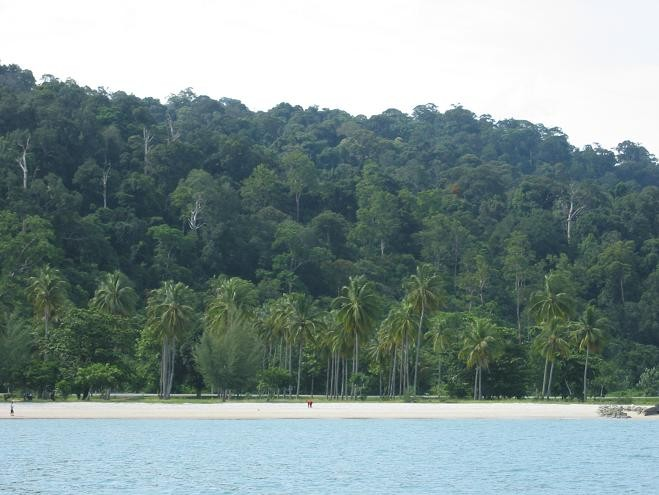
\includegraphics[width=4.8cm]{articles/langkawi/1211018197eneE.jpg}
Plage de Langkawi

\hspace*{-0.65cm}
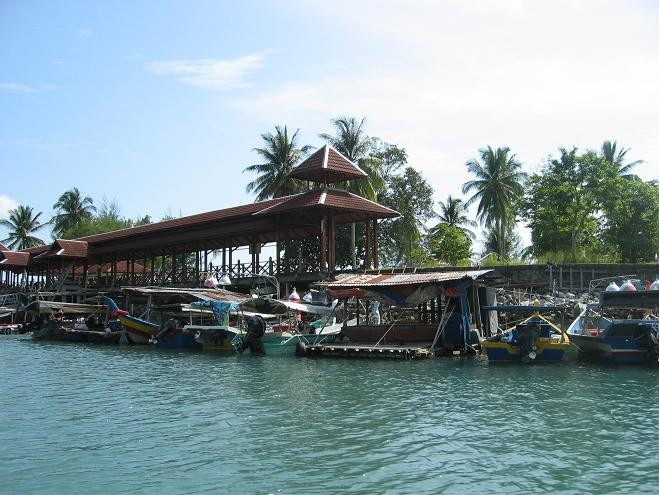
\includegraphics[width=4.8cm]{articles/langkawi/1211018204F7Ee.jpg}
Entrée de la marina

\hspace*{-0.65cm}
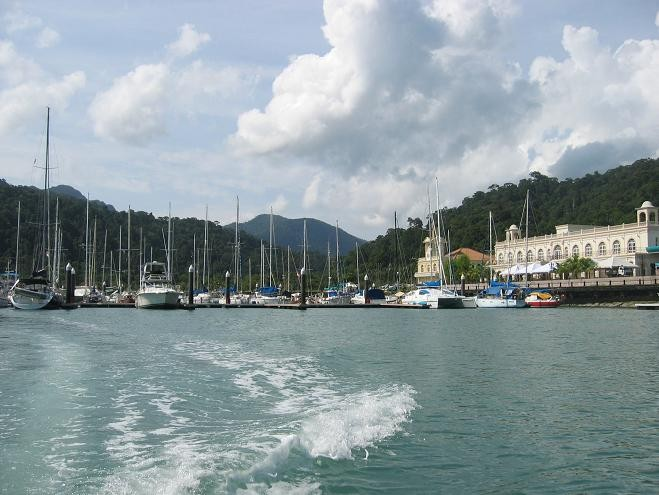
\includegraphics[width=4.8cm]{articles/langkawi/1211018457DniB.jpg}
Ben... sortie de la marina... le même endroit, quoi

Et c'est parti pour visiter, pas loin de la marina il y a des chutes d'eau. On voulait au depart aller prendre un télépherique qui monte au sommet de la colline pour voir toute l'île mais il était en réparation, ce n'est que partie remise.

\hspace*{-0.65cm}
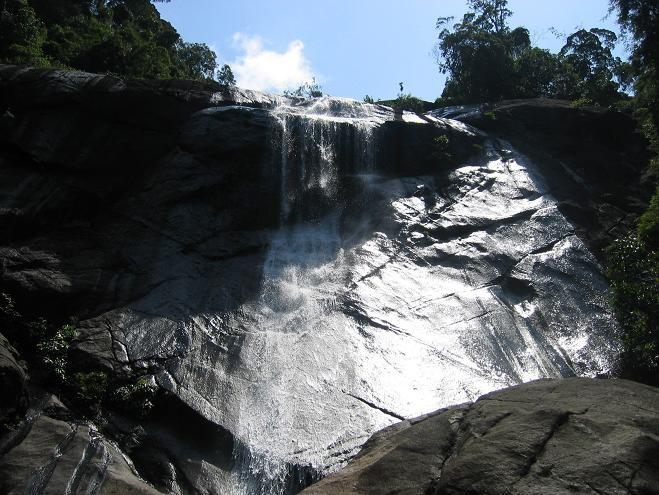
\includegraphics[width=4.8cm]{articles/langkawi/1211018190Pmip.jpg}
Cascade

Je complèterai cet article dans les jours qui viennent avec des photos du tour de l'île, je vais louer un scooter car il parait que ça vaut vraiment le coup a faire...

Je vous laisse sur une petite note poissonistique.

%<div><object width="640" height="505"><param name="movie" value="http://www.dailymotion.com/swf/x5gab6&v3=1&related=1"></param><param name="allowFullScreen" value="true"></param><param name="allowScriptAccess" value="always"></param><embed src="http://www.dailymotion.com/swf/x5gab6&v3=1&related=1" type="application/x-shockwave-flash" width="640" height="505" allowFullScreen="true" allowScriptAccess="always"></embed></object></div>

Voici comme promis quelques photos en plus.

\hspace*{-0.65cm}
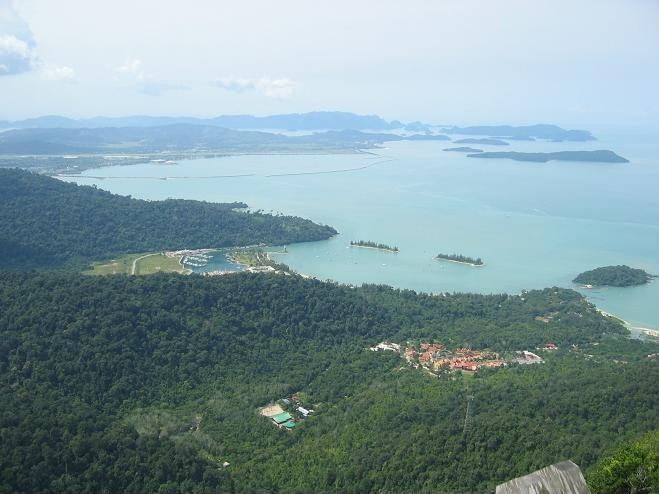
\includegraphics[width=4.8cm]{articles/langkawi/1212397933wQ6v.jpg}
La marina vue d'en haut

\hspace*{-0.65cm}
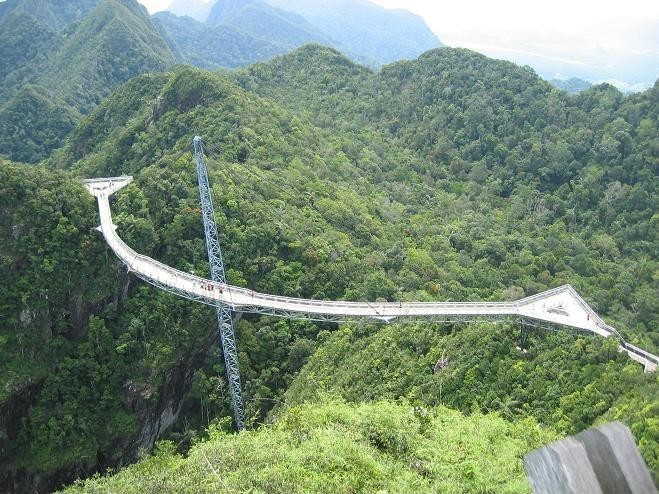
\includegraphics[width=4.8cm]{articles/langkawi/1212398042f2k1.jpg}
Une passerelle touristique

\hspace*{-0.65cm}
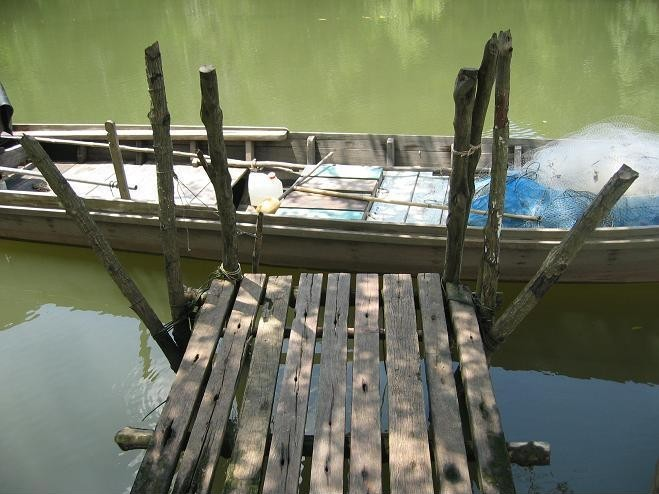
\includegraphics[width=4.8cm]{articles/langkawi/1212397931akoQ.jpg}
Petit ponton dans la mangrove

PS : N'oubliez pas d'aller voir l'article sur Kuala Lumpur que je viens d'écrire juste avant.

PS2 : Vous remarquerez la présence maintenant d'un contrôle anti-spam qu'il est obligatoire de remplire si vous voulez laisser un commentaire, c'est triste de devoir mettre ça en place mais vu les !$%&!! de messages qui arrivaient en masse ces derniers temps je n'ai pas le choix, en espérant que ça résolve le problème.

TODO : Peut virer les PS

\end{multicols}
